\documentclass[11pt]{article}
\usepackage[top=1in, bottom=0.5in, left=1in, right=1in]{geometry}
\usepackage[T1]{fontenc}
\usepackage[polish]{babel}
\usepackage[utf8]{inputenc}
\usepackage{lmodern}
\selectlanguage{polish}
\usepackage{graphicx}
\begin{document}
\title{Laboratorium 8}
\author{Jan Seredyński}
\date{\today}
\maketitle

\section{Wstęp}
Zadaniem laboratorium jest pomiar czasu wykonania operacji dodawania, wyszukania elementów z drzewa binarnego, z implementacja AVL.\\\
Drzewo AVL pozostaje drzewem BST, co oznacza, że wierzchołki są uporządkowane w określony sposób. Zazwyczaj przyjmuje się, iż elementy w lewym poddrzewie są mniejsze od wierzchołka, zaś w prawym - większe. Zrównoważenie drzewa osiąga się przypisując każdemu węzłowi współczynnik wyważenia, który jest równy różnicy wysokości lewego i prawego poddrzewa. Może wynosić 0, +1 lub -1. Wstawiając lub usuwając elementy drzewa (tak aby zachować własności drzewa BST) modyfikuje się też współczynnik wyważenia, a gdy przyjmie on niedozwoloną wartość wykonuje specjalną operację rotacji węzłów, która przywraca zrównoważenie. Wysokość drzewa AVL gwaratnuje złożoność obliczeniową wysokości O(log n)\\\
gdzie wsp wyważenia = wysokoscLewego(w) - wysokoscPrawego(w)


\section{Wyszukiwanie elementu}
Wyszukiwanie elementu w drzewie AVL nie różni się od BST. Jego złożoność w teori wynosi w log(n). Na moim wykresie logarytmicznym można zaobserowawać, że w algorytm w rzeczywistości pracował z gorszą wydajością - liniowa O(n), co mogło być spowodowane
złymi strukturami w programie lub równoległymi procesami.Pomimo tych niedogodności można zauważyć jak bardzo uporządkowane drzewo AVL ma mniejszą złożoność obliczeniową od BST, co przedstawia poniżysz wykres.
\par\vspace{\baselineskip}
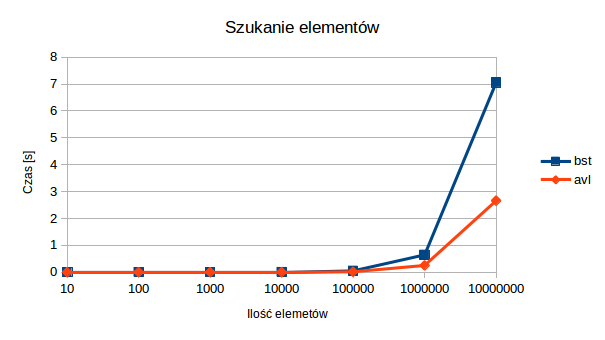
\includegraphics[width=5in]{wysz.png}\\\
\newpage



\section{Dodawanie elementu}
Dodawanie gałęzi w drzewie polega na implementacji rotacji, czyli takich przestawień elementów, aby odpowiednie gałęzie byly odpowiednio zbalansowane. Wyróżniamy dwa typy rotacji LL rotacja w prawo (elementy połączone lewymi odnogami) i RR rotacja w lewo (prawymi odnogami). Możemy wyróżnić jeszcze dwie RL,LR są to rotacje podwójne, które składają się właśnie z kombinacji rotacji LL i RR.  \\\
Złożoność obliczeniowa dodawania gałęzi w drzewie AVL jest większa niż w BSD ponieważ trzeba dodatkowo balansować drzewo. Jednak jak widać z wykresu jest to mała strata w porównaniu do złożoności którą możemy odzyskać podczas  wykukiwania elemntów.\\\
Złożoność obliczeniowa dodawania elementów w teroi wynosi O(log n).

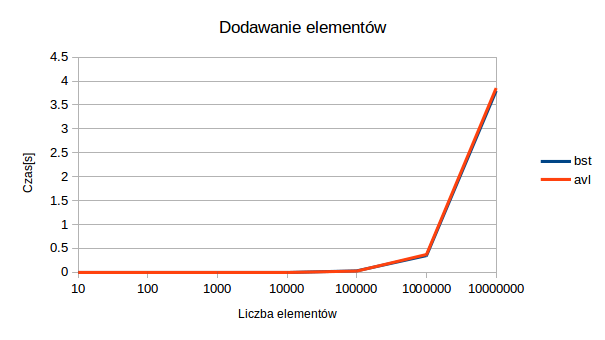
\includegraphics[width=5in]{dod.png}\\\




\section{Podsumowanie}
Drzewo AVL charakteryzuje się większą złożonością obliczeniową od BSD w przypadku wsadzania elementów, natomiast jest zdecydowanie wydajniejsze podczas wyszukiwania elementów.
\end{document}